%%%%%%%%%%%%%%%%%%%%%%%%%%%%%%%%%%%%%%%%%%%%%%%%%%%%%%%%%%%%%%%%%%%%%%%%%%%%
% AGUtmpl.tex: this template file is for articles formatted with LaTeX2e,
% Modified September 2012
%
% This template includes commands and instructions
% given in the order necessary to produce a final output that will
% satisfy AGU requirements.
%
% PLEASE DO NOT USE YOUR OWN MACROS
% DO NOT USE \newcommand, \renewcommand, or \def.
%
% FOR FIGURES, DO NOT USE \psfrag or \subfigure.
%
%%%%%%%%%%%%%%%%%%%%%%%%%%%%%%%%%%%%%%%%%%%%%%%%%%%%%%%%%%%%%%%%%%%%%%%%%%%%
%
% All questions should be e-mailed to latex@agu.org.
%
%%%%%%%%%%%%%%%%%%%%%%%%%%%%%%%%%%%%%%%%%%%%%%%%%%%%%%%%%%%%%%%%%%%%%%%%%%%%
%
% Step 1: Set the \documentclass
%
% There are two options for article format: two column (default)
% and draft.
%
% PLEASE USE THE DRAFT OPTION TO SUBMIT YOUR PAPERS.
% The draft option produces double spaced output.
%
% Choose the journal abbreviation for the journal you are
% submitting to:

% jgrga JOURNAL OF GEOPHYSICAL RESEARCH
% gbc   GLOBAL BIOCHEMICAL CYCLES
% grl   GEOPHYSICAL RESEARCH LETTERS
% pal   PALEOCEANOGRAPHY
% ras   RADIO SCIENCE
% rog   REVIEWS OF GEOPHYSICS (if you encounter problems with this class file, use jgrga instead)
% tec   TECTONICS
% wrr   WATER RESOURCES RESEARCH
% gc    GEOCHEMISTRY, GEOPHYSICS, GEOSYSTEMS
% sw    SPACE WEATHER
%
% For JOURNAL OF ADVANCES IN MODELING EARTH SYSTEMS, use jgrga.
%
%
% (If you are submitting to a journal other than jgrga,
% substitute the initials of the journal for "jgrga" below.)

\documentclass[draft,jgrga]{agutex}

%%%%%%%%%%%%%%%%%%%%%%%%%%%%%%%%%%%%%%%%%%%%%%%%%%%%%%%%%%%%%%%%%%%%%%%%%
% OPTIONAL:
% To produce a two-columned version:
%\documentclass[jgrga]{AGUTeX}

% Two-columned format can be used to estimate the number of pages
% for the final published PDF.

% PLEASE USE THE DRAFT OPTION TO SUBMIT YOUR PAPERS.
%%%%%%%%%%%%%%%%%%%%%%%%%%%%%%%%%%%%%%%%%%%%%%%%%%%%%%%%%%%%%%%%%%%%%%%%%
% OPTIONAL:
% To create numbered lines:

% If you don't already have lineno.sty, you can download it from
% http://www.ctan.org/tex-archive/macros/latex/contrib/ednotes/
% (or search the internet for lineno.sty ctan), available at TeX Archive Network (CTAN).
% Take care that you always use the latest version.

% To activate the commands, uncomment \usepackage{lineno}
% and \linenumbers*[1]command, below:

\usepackage{lineno}
\linenumbers*[1]

%  To add line numbers to lines with equations:
% \begin{linenomath*}
%\begin{equation}
%\end{equation}
%\end{linenomath*}
%%%%%%%%%%%%%%%%%%%%%%%%%%%%%%%%%%%%%%%%%%%%%%%%%%%%%%%%%%%%%%%%%%%%%%%%%
% Figures and Tables
%
% When submitting articles through the GEMS system:
% COMMENT OUT ANY COMMANDS THAT INCLUDE GRAPHICS.
% (See FIGURES section near the end of the file.)
%
% DO NOT USE \psfrag or \subfigure commands.
%
%  Figures and tables should be placed AT THE END OF THE ARTICLE,
%  after the references.
%
%  Uncomment the following command to include .eps files
%  (comment out this line for draft format):
\usepackage{graphicx}
%
%  Uncomment the following command to allow illustrations to print
%   when using Draft:
%\setkeys{Gin}{draft=True}
%
% Substitute one of the following for [dvips] above
% if you are using a different driver program and want to
% proof your illustrations on your machine:
%
% [xdvi], [dvipdf], [dvipsone], [dviwindo], [emtex], [dviwin],
% [pctexps],  [pctexwin],  [pctexhp],  [pctex32], [truetex], [tcidvi],
% [oztex], [textures]
%
% See how to enter figures and tables at the end of the article, after
% references.
%
%%%%%%%%%% Start TeXmacs macros
\usepackage{amsmath,bbm}
\newcommand{\nonesep}{}
\newcommand{\tmem}[1]{{\em #1\/}}
\newcommand{\tmop}[1]{\ensuremath{\operatorname{#1}}}
\newcommand{\tmsamp}[1]{\textsf{#1}}
\newcommand{\tmstrong}[1]{\textbf{#1}}
\newcommand{\tmtextit}[1]{{\itshape{#1}}}
\newcommand{\parby}[2]{\ensuremath{\frac{\partial #1}{\partial #2}}}
\newcommand{\E}{\ensuremath{\vec{E}}}
\newcommand{\V}{\ensuremath{\vec{v}}}
\newcommand{\U}{\ensuremath{\vec{u}}}
\newcommand{\B}{\ensuremath{\vec{B}}}
\newcommand{\J}{\ensuremath{\vec{J}}}
\newcommand{\Vper}{\ensuremath{\vec{v}_{\perp}}}
\newcommand{\Vpara}{\ensuremath{\vec{v}_{\parallel}}}
\newcommand{\Uper}{\ensuremath{\vec{u}_{\perp}}}
\newcommand{\Upara}{\ensuremath{\vec{u}_{\parallel}}}
\newcommand{\X}{\ensuremath{\vec{x}}}
\newcommand{\DIV}{\ensuremath{\nabla \cdot}}
\newcommand{\CURL}{\ensuremath{\nabla \times}}
%%%%%%%%%% End TeXmacs macros
\usepackage{setspace}
%% ------------------------------------------------------------------------ %%
%
%  ENTER PREAMBLE
%
%% ------------------------------------------------------------------------ %%

% Author names in capital letters:
\authorrunninghead{WILTBERGER ET AL.}


% Shorter version of title entered in capital letters:
\titlerunninghead{Effects of AEH}

%Corresponding author mailing address and e-mail address:
%\authoraddr{Corresponding author: A. B. Smith,
%Department of Hydrology and Water Resources, University of
%Arizona, Harshbarger Building 11, Tucson, AZ 85721, USA.
%(a.b.smith@hwr.arizona.edu)}
\authoraddr{Corresponding author: M. Wiltberger,
National Center for Atmospheric Research,
High Altitude Observatory,
3080 Center Green,
Boulder, CO 80301
(wiltbemj@ucar.edu)}
\paperid{???}
\begin{document}

\def\oplus{O$^+$ }
\def\hplus{H$^+$ }
\def\heplus{He$^+$}
\def\nplus{N$^+$}
\def\dst{$D_{ST}$ }


%% ------------------------------------------------------------------------ %%
%
%  TITLE
%
%% ------------------------------------------------------------------------ %%


\title{Effects of Anomalous Electron Heating in simulations of the March 17, 2013 Geomagnetic Storm}
%
% e.g., \title{Terrestrial ring current:
% Origin, formation, and decay $\alpha\beta\Gamma\Delta$}
%

%% ------------------------------------------------------------------------ %%
%
%  AUTHORS AND AFFILIATIONS
%
%% ------------------------------------------------------------------------ %%


%Use \author{\altaffilmark{}} and \altaffiltext{}


% \altaffilmark will produce footnote;
% matching \altaffiltext will appear at bottom of page.

% \authors{A. B. Smith,\altaffilmark{1}
% Eric Brown,\altaffilmark{1,2} Rick Williams,\altaffilmark{3}
% John B. McDougall\altaffilmark{4}, and S. Visconti\altaffilmark{5}}

%\altaffiltext{1}{Department of Hydrology and Water Resources,
%University of Arizona, Tucson, Arizona, USA.}

%\altaffiltext{2}{Department of Geography, Ohio State University,
%Columbus, Ohio, USA.}

%\altaffiltext{3}{Department of Space Sciences, University of
%Michigan, Ann Arbor, Michigan, USA.}

%\altaffiltext{4}{Division of Hydrologic Sciences, Desert Research
%Institute, Reno, Nevada, USA.}

%\altaffiltext{5}{Dipartimento di Idraulica, Trasporti ed
%Infrastrutture Civili, Politecnico di Torino, Turin, Italy.}

\authors{M. Wiltberger, \altaffilmark{1}
V. Merkin, \altaffilmark{2}
B. Zhang,   \altaffilmark{1}
F. Toffletto,  \altaffilmark{3}
M. Oppenheim,  \altaffilmark{4}
W. Wang,  \altaffilmark{1}
J. G. Lyon, \altaffilmark{5}
J. Liu,  \altaffilmark{1}
and Y Dimant \altaffilmark{4}
}

\altaffiltext{1}
{High Altitude Observatory, National Center for Atmospheric Research,Boulder, Colorado, USA.}

\altaffiltext{2}{Applied Physics Laboratory, Johns Hopkins University, MD, USA.}

\altaffiltext{3}{Department of Physics and Astronomy, Rice University, TX, USA.}

\altaffiltext{4}{2Center for Space Physics, Boston University, Boston, Massachusetts, USA}

\altaffiltext{5}{Department of Physics and Astronomy, Dartmouth College,Hanover, NH, USA.}
%

%% ------------------------------------------------------------------------ %%
%
%  ABSTRACT
%
%% ------------------------------------------------------------------------ %%

% >> Do NOT include any \begin...\end commands within
% >> the body of the abstract.

\begin{abstract}
Examines the impacts of including Anomalous Electron Heating (AEH) in simulations of to the geomagnetic storm that occurred on 17 March 2013.   We see many cool things.

\end{abstract}

%% ------------------------------------------------------------------------ %%
%
%  BEGIN ARTICLE
%
%% ------------------------------------------------------------------------ %%

% The body of the article must start with a \begin{article} command
%
% \end{article} must follow the references section, before the figures
%  and tables.

\begin{article}

%% ------------------------------------------------------------------------ %%
%
%  TEXT
%
%% ------------------------------------------------------------------------ %%

\section{Introduction}

Initial drafting of this section has been assigned to Meers and Slava.

\section{Simulation Setup}
\label{sec-model-sims}
This study focuses on using the geomagnetic storm that occurred on 17 March 2013 as a case study for two new features of the LFM-RCM geospace model.   As previously discussed the LFM-RCM model combines the Lyon-Fedder-Mobarry MHD model of the magnetosphere with the Rice Convection Model of the inner magnetosphere and the Mangetosphere-Ionosphere Coupler Solver of ionospheric electrodynamics to provide a tightly coupled model of the geospace system. \cite{Pembroke:2012gc} describes in detail the basic process of coupling these three models together during idealized solar wind conditions with modest solar wind driving and no dipole tilt.  Section \ref{sec-lfm-rcm} describes how this approach has been modified to include realistic solar wind conditions, including nonzero IMF $B_Y$, as well as variations in the Earth's dipole tilt.  \cite{2005GeoRL..3222101M} implemented an adjustment to the ionospheric conductances based upon the theoretical analysis of the Farley-Buneman instability (FBI) conducted by \cite{2003JGRA..108.1350D}.  This capability has not be widely used in LFM simulations, but is being made part of the LFM-RCM geospace model.  Section \ref{sec-aeh} discusses how both the Anomalous Electron Heating (AEH) and Non-Linear Current (NLC) aspects of the FBI are implemented in the MIX portion of the LFM-RCM model.  In the final section of the portion of  the paper we present the solar wind conditions present during the 17 March 2013 geomagnetic storm and document the specific details of the LFM-RCM simulation chosen for this event study.

\subsection{LFM-RCM}
\label{sec-lfm-rcm}

\cite{Pembroke:2012gc} provides a detailed description of the coupling process between the LFM, MIX and RCM models for simulations of geospace.  Since that study used idealized solar wind conditions with no dipole tilt after reviewing the basics of the LFM-RCM coupling this section will address the changes made to coupling infrastructure needed to allow model to work for realistic solar wind conditions and dipole tilts.  

The fundamental aspect of the model coupling is an exchange of magnetic field and plasma information in the inner magnetosphere to RCM from LFM and then an update of the plasma information from RCM to the LFM.  The MIX model is providing ionospheric potential information to both the LFM and RCM models.  All of the exchanges use the Center for Integrated Space Weather Modeling (CISM) \cite{2004JASTP..66.1469G} coupling infrastructure  and that infrastructure is utilized in the update version.  To transfer information from the LFM to the RCM it computes time averages of the pressure, density and magnetic field over an exchange interval.  This intermediate grid is then used to calculated field line-averaged pressure and density for positions in the RCM's ionospheric grid.  A key innovation of the \cite{Pembroke:2012gc} was the implementation of the plasma-$\beta$ methodology for setting the location of the outer boundary of the RCM.  This switch, which essentially prevented the RCM from computing regions with large flows, remains active in the storm simulations we present in this paper.  The averaged fields are interpolated onto an intermediate regular Cartesian grid. After the RCM computes its plasma pressures and densities these values are transferred back to the LFM once again using the intermediate grid.  The RCM density model includes a modifications to a fit of static plasmasphere model of \cite{Gallagher:2000p2797}.  At this time we have not implemented a dynamic plasmasphere calculation, but that is logical next step for improvement of the coupled model.  Another set of field line traces from the RCM ionospheric grid points are used to determine the local values on intermediate grid and than those values are interpolated to LFM grid points.  The mapping back to LFM assumes that the distribution of plasma density and pressure  is constant along field lines. As before the RCM values do not immediately replace the LFM values, instead they bled into the LFM over the exchange time interval.  It is important to note that the previous work used a 1-minute exchange interval as a  balance between speed and accuracy.  For strong solar wind driving conditions we have found it necessary to reduce the coupling interval to 15-seconds. 

The first major modification to the previous coupling efforts is in support of including dipole tilts in the calculation of the coupled model.  The LFM-MIX model has long had support for conducting simulations with realistic dipole tilts.  This is done by continuing to have the dipole axis of the Earth aligned with the Z-axis of the computational model and inputing the solar wind conditions in SM coordinates.  As \cite{1992P&SS...40..711H} explains the SM coordinate system has the Z-axis parallel to the north magnetic pole and transformation between this coordinate system and the more commonly used GSM coordinate system is simply rotation about the Y-axis by the dipole tilt angle.   The cartesian intermediate grid is setup in SM coordinates for the transfer of data to and from the LFM to RCM the ionospheric foot points are transformed from geographic coordinates to SM coordinates using the GEOPACK coordinate transform package.    While the RCM typically includes the effects of the corotation potential since this is not enabled in the LFM-MIX simulation these effects are disabled within the RCM when it is coupled to the LFM.  

The second key modification of the LFM-RCM coupling is how the asymmetries in the ionosphere are addressed.  In the MIX module the ionospheric potential for the northern and southern hemispheres are calculated independently.  The field-aligned current patterns are taken from the global MHD simulation are shared between the hemispheres, but the ionospheric conductances can be different.  The first major difference comes from the implementation the EUV conductance model that calculates the local value of the Hall and Pedersen conductance based upon the solar zenith angle and the F107 flux value.  We have adapted the model used by AMIE for the MIX module \cite{1992AdSpR..12...59R}.  The ionospheric conductance model also includes an empirical model for electron precipitation.  As described by \cite{2009JGRA..11401204W} this model includes modifications of the precipitation values based upon the local EUV conductance values allowing the model to simulate seasonal variations of particle precipitation and their impacts on geospace system.  On the other hand the RCM assumes that there are no differences between the northern and southern hemispheres.  

The compromise solution we have adopted for the version of the coupled simulations present here works as follows.  The low latitude boundary of the the ionospheric solution for electrodynamic solve is extended equatorward for 45$\circ$ to 60$\circ$ colatitude.   The 45$\circ$ boudnary corresponds to dipole mapping of the 2 $R_E$ inner boundary of the MHD solution grid within the LFM.  The 60$\circ$ boundary corresponds to the low latitude boundary for the RCM ionospheric calculation. {\em Frank - Is the previous statement correct?} For the northern hemisphere the typical low latitude boundary condition of assuming that potential is zero is used.  The northern hemispheric values for the potential as well as the average energy and flux of precipitating electrons are then stored for latter passage to the RCM for its calculation.  The computation of the southern hemisphere potential is done down 45$\circ$ with the low latitude boundary value being set of the potential obtained from the northern hemisphere at that location.   By setting the southern hemisphere boundary with the northern hemisphere values we are attempting ensure that closed field lines in the calculation have the same potential values.   {\em Slava and Frank - Is that the best way to describe the motivation for this coupling approach?  Also, should we address why we aren't passing any kind of aggregate flux or conductance information to the RCM calculation.}

As a quick side note we take a moment to compare our approach that utilized by the Space Weather Modeling Framework \cite{2005JGRA..11012226T} to couple the MHD magnetosphere solution to inner magnetosphere models.   \cite{2004JGRA..10912219D} did the initial work coupling the RCM with the BATS-R-US magnetosphere solution.  Like us they used field line tracing to compute flux tube quantities for transfer between the two components and also assume the plasma parameters are constant along field lines.  They support coupling intervals between 10 seconds to 10 minutes with coupling time between models with balance being driving by the strength of  convection within the event being simulated.  This initial work was done for simulations with no dipole tilts and uniform ionospheric conductances.   \cite{2010SpWea...803002W} presents validation studies comparing the magnetic field and plasma parameters for a set of geomagnetic storms.  While these results clearly include the effects of dipole tilts and particle precipitation effects the study does not provide any details on how these conditions are handed in the coupled model.   More recently \cite{Glocer:2013dv} documented the two-way coupling of the Comprehensive Ring Current Model (CRCM) with the BATS-R-US global magnetosphere model, while they presented results for 22 July 2009 geomagnetic storm the paper does not discuss the details of how dipole tilt are addressed.  {\em Frank and Slava - I thought this was a worth while addition here and not in the introduction since it concentrates on coupling details.  Am I being to harsh in my language about not discussing how the dipole tilt is addressed? I'm not aware of any OpenGGCM publications with RCM.  If I've missed something please let me know.}

\subsection{FBI Implementation}
\label{sec-aeh}

\cite{2011JGRA..116.9304D} developed a model for including the effects that plasma turbulence can have on E-region conductivities in regions of strong DC electric fields.  This tublence can drive nonlinear currents and have strong anomalous electron heating of the plasma.  Both these effects can enhance the conductivity.  Their model provides correction factors for the conductivities that we have implemented into the MIX module.

{\em Meers and Yakov - Please insert a paragraph or two with more background information. In particular, I need justification for why we are only applying this regions with E greater than 35 mV/m}  

Inside the MIX module we have implemented the following conductivity correction terms.   In regions where the electric field is greater than 35 mV/m we have implemented, 

\begin{equation}
\label{eq-sigmap-fbi}
\Sigma_P^{FBI} = \Sigma_P^O(1+0.01 (E - 35) + 1.3e10^{-5}(E - 35)^2),
\end{equation}

as the calculation for the FBI modified conductivity, $\Sigma_P^{FBI}$.  In Equation \ref{eq-sigmap-fbi} $E$ is the ionospheric electric field in mV/m and $\Sigma_P^O$ is the Pedersen conductivity obtained from the baseline ionospheric model and includes both the EUV and electron precipitation terms.  This multiplier includes the effect of the temperature driven recombination reduction as well as the that of nonlinear current.  The FBI modified Hall conductivity, $\Sigma_H^{FBI}$ ,  is simply 

\begin{equation}
\label{eq-sigmah-fbi}
\Sigma_H^{FBI} = \Sigma_H^O(1+0.01172 (E - 35) - 1.207e10^{-5}(E - 35)^2),
\end{equation}

where $\Sigma_H^O$ is the baseline Hall conductivity.   Figure \ref{fbi-multi-fig} shows the effects of these multipliers over a range electric fields.  The Pedersen multiplier (blue curve) is nearly linear over the range from 35-200 mV/m reaching a peak value of 3.0 at 200 mV/m.  The Hall multiplier has a negative coefficient on the the squared term and so falls of more dramatically at higher values of the electric field.  It reaches a peak value of 2.3 at 200 mV/m.  {\em Meers and Yakov - Not sure if the figure adds much, but I'm happy to include it.}

\begin{figure}
\noindent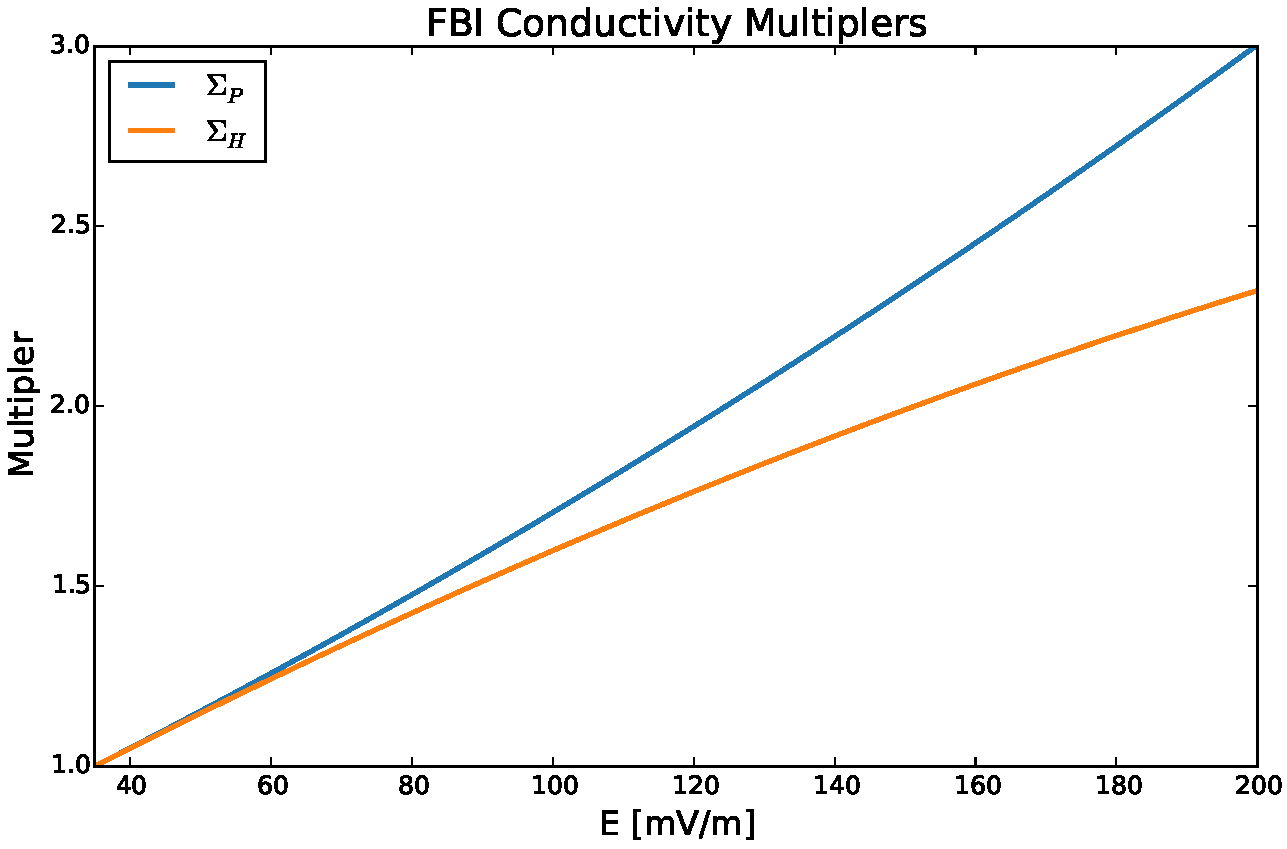
\includegraphics[width=20pc]{JGRPaper-ConductMulti.pdf}
\caption{\label{fbi-multi-fig} 
The conductivity multipliers for the FBI effects.  The blue curve is for the Pedersen conductivity while the orange curve is for the Hall conductivity.  The effects occur for all values above 35 mV/m.  } 
\end{figure}

\subsection{17 March 2013 Simulation}
\label{sec-17mar13}

On 17 March 2013 an interplanetary coronal mass ejection arrived at the Earth and drove a significant geomagnetic storm, $D_{ST} < -100$, over the next day.  Solar wind conditions obtained from the OMNI dataset where used to drive the LFM-RCM model and those are shown in Figure \ref{sw-fig}.  Prior to the shock preceding the CME the solar wind conditions are fairly typical, namely density ~ 5 cc, velocity ~ 425 km/s, with interplanetary magnetic field (IMF) weak, $<$ 5nT in magnitude, main in the northward direction.  At 05:55 UT a shock is clearly present in the solar wind with $V_X$ GSM reaching -650 km/s and the density increasing to 10 cc.  In the next three hours the IMF is variable, with IMF $B_Z$ mainly southward reaching values of -20 nT, but having significant intervals with northward IMF.  The Y component of the IMF has similar magnitude in amplitude and appears to have a 180 $\deg$ phase shift.  After approximately  09:00 UT on the 17th the Y and Z components become more in phase and slowly reduce in amplitude reaching typical values by the end of the day.  After about 12:00 UT the solar wind speed slowly begins to decrease reaching a value of about 550 km/s by the end of 17 March.

The LFM-RCM simulations for this interval where run using solar wind conditions from Figure \ref{sw-fig}.  As previously discussed the LFM uses a non-orthogonal spherical mesh for the grid.  The simulations conducted here use 106 radial, 96 azmiuthal, and 128 polar cells.  This quad resolution version of the LFM contains twice as many cells as the results reported by \cite{Pembroke:2012gc} initial work with coupling LFM-RCM.   The RCM simulations where done on a grid with XX and YY points.  The intermediate transfer grid between LFM-RCM used for the field line tracing had a resolution of ZZ.  In the MIX ionospheric solution the ionospheric resolution was increased from a 2x2$^{\circ}$ resolution to 1x1$^{\circ}$resolution.  The full ionospheric conductance model described by \cite{2009JGRA..11401204W} by was enabled in the MIX calculations.  We ran two sets of simulations.  The first hereafter, baseline, used the standard ionospheric model.  The second, hereafter AEH, had the AEH implementation discussed in Section \ref{sec-aeh} enabled.  The solar wind driving, grid resolution, and all other model parameters are not changed between these to runs. 

\begin{figure}
\noindent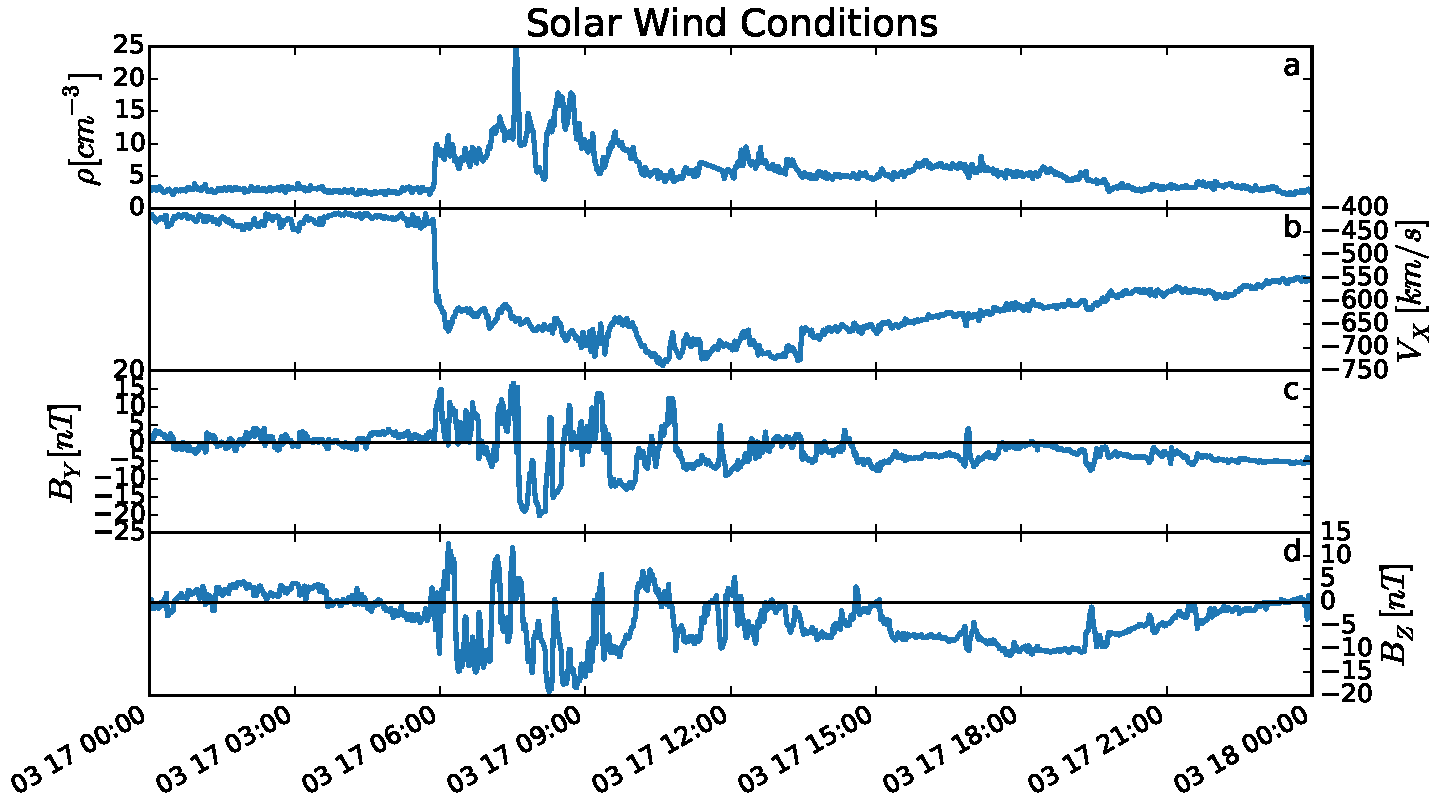
\includegraphics[width=20pc]{JGRPaper-SWFig.pdf}
\caption{\label{sw-fig} 
Solar wind and IMF conditions during the 17 March 2013 geomagnetic storm event.  Panel a) shows the number density, b) the $V_X$ in GSM coordinates.  The IMF GSM Y and Z values are plotted in panels c) and d) respectively.} 
\end{figure}

\section{Analysis of results}
\label{sec-analysis}
In this section we examine impact of the using AEH.

\subsection{Baseline versus AEH}

Initial drafting of this section is assigned to Mike.

Possible figures include 

\begin{figure*}[t]
\noindent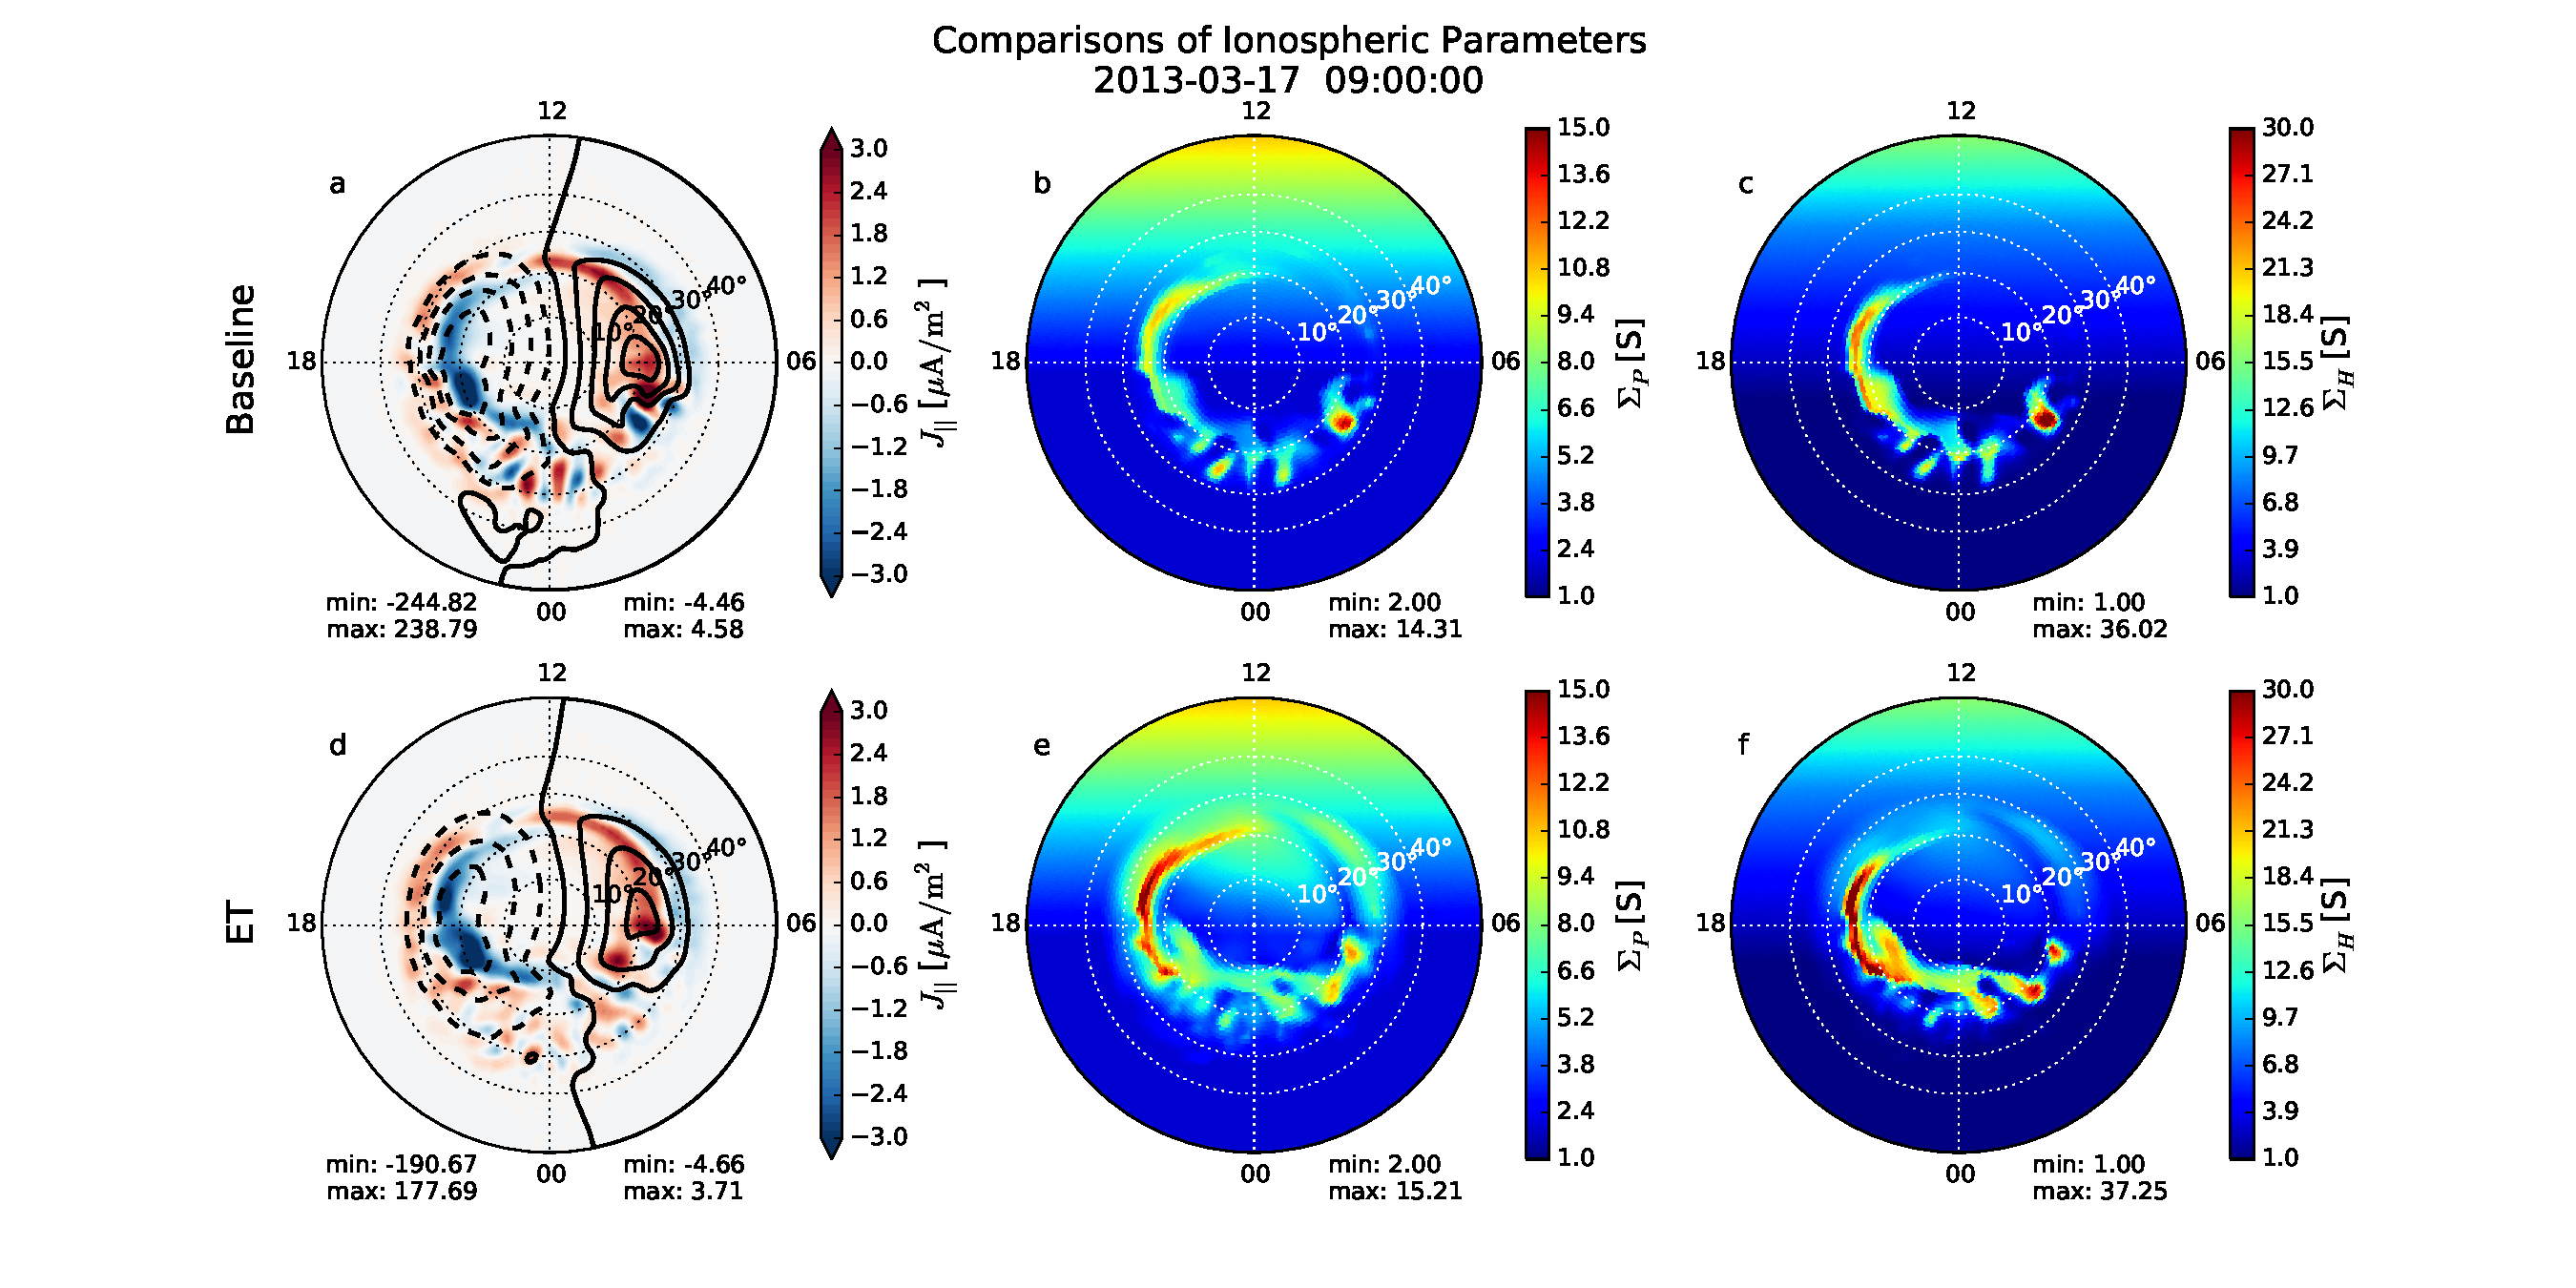
\includegraphics[width=39pc]{JGRPaper-IonPatterns.pdf}
\caption{\label{ion-comp-fig}
Comparison of FAC and CPCP as well as Pedersen and Hall conductivities for the Baseline and AEH simulations of the 17 March 2016 geomagnetic storm.  The top row (panels a-c) contains the results from the baseline simulation while the bottom row (panels d-f) contains the results of the simulation with the AEH enabled.  The first column (panels a and d) has the FAC in color with blue being upward and red being downward as well as the CPCP pattern with 20 kV contours.  The middle column (panels b and e) contains the Pedersen conductivity.  The last column (panels c and f) contains the Hall conductivity.  The colorbar for all conductivity plots is the same.}
\end{figure*}

\begin{figure}
\noindent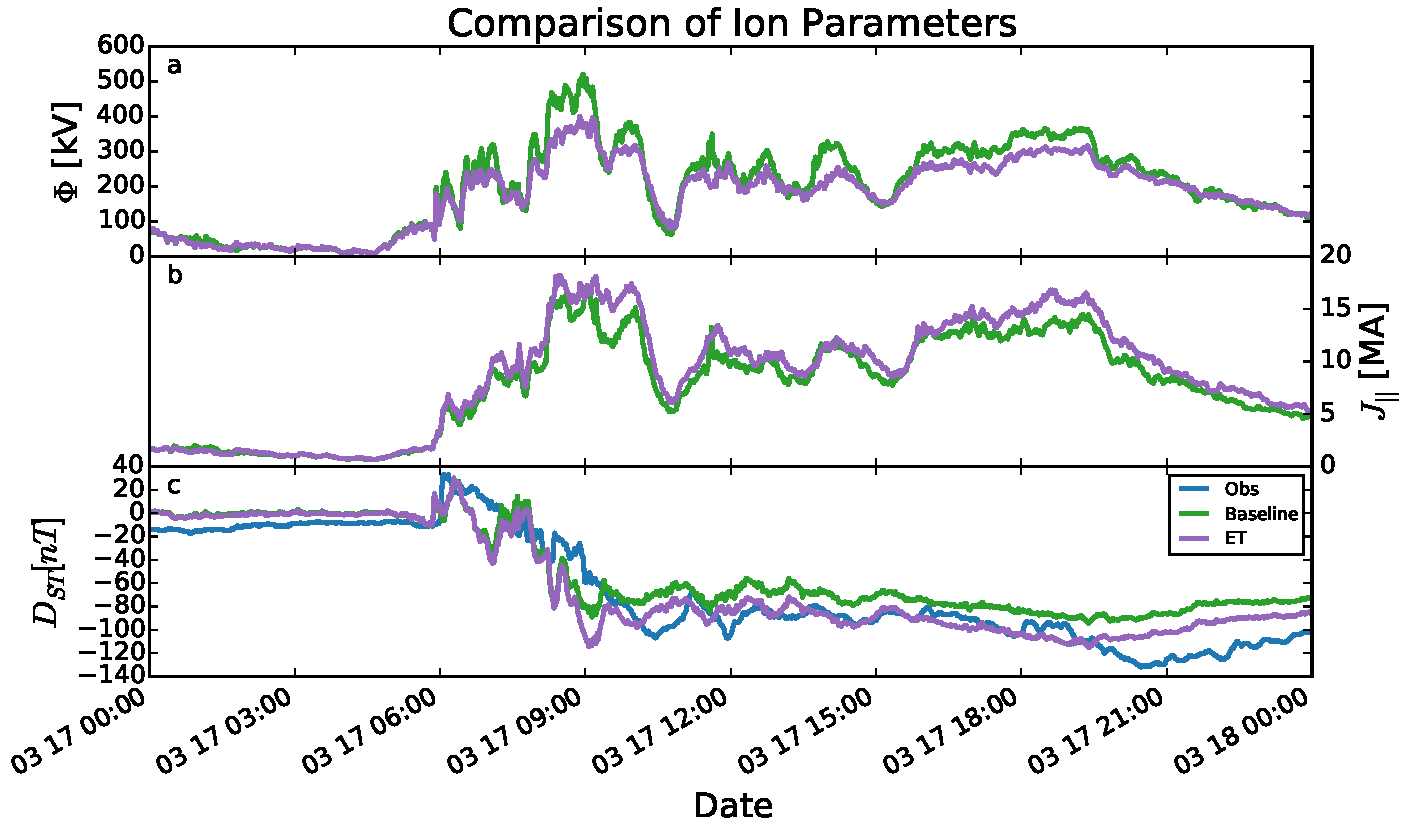
\includegraphics[width=20pc]{JGRPaper-IonFig.pdf}
\caption{\label{ts-fig} 
Comparison of the CPCP, FAC, and $D_{ST}$ time series for the storm event for the Northern hemisphere .  Panel a at the top shows the CPCP in kV.  The middle panel (b) has the integrated  FAC.  Panel c at the bottom has the $D_{ST}$ index.  In each panel the LFM-RCM results are shown with the green line, the AEH results with the purple line.  In the bottom panel the $D_{ST}$ obtained from CDAWeb is plotted in blue} 
\end{figure}

 \subsection{Comparison with DSMP}
Initial drafting of this section has been assigned to Bin.
 
 \begin{figure*}[t]
\noindent\includegraphics[width=39pc]{DMSPTraj.pdf}
\caption{\label{dmsptraj-fig}
DSMP F17 and F18 trajectories overlaid ontop of AEH FAC and CPCP patterns.  Panel a shows the F17 trajectory between 0945 and 1030 UT and the F18 trajectory beteween 1000 and 1045 UT overlaid on top of the AEH simulation results for 10:00UT.   Panel b shows the F17 trajectory between 1125 and 1210 UT and the F18 trajectory beteween 1145 and 1230 UT overlaid on top of the AEH simulation results for 12:00UT.  In each panel the F17 trajectory is pink and the F18 trajectory is blue.}
\end{figure*}

\begin{figure*}[t]
\noindent\includegraphics[width=39pc]{DMSP_F17_AEH_compare.png}
\caption{\label{f17-comp-fig}
Temporary Figure comparing DMSP F17 results. }
\end{figure*}

\begin{figure*}[t]
\noindent\includegraphics[width=39pc]{DMSP_F18_AEH_compare.png}
\caption{\label{f18-comp-fig}
Temporary Figure comparing DMSP F18 results}
\end{figure*}

 \subsection{Comparison with AMPERE}
 
 Initial drafting of this section has been assigned to Mike.
 
 Here will discuss the results and compare them with AMPERE
 
\begin{figure*}[t]
\noindent\includegraphics[width=39pc]{AmpereComparison.pdf}
\caption{\label{ampere-comp-fig}
Temporary Figure comparing AMPERE and LFM-RCM}
\end{figure*}

 \subsection{Comparison with TS07-D}
 
 Initial drafting of this section has been assigned to Slava.
 
 
 May include a comparison with pressures in the in the ring current depending on length and quality of comparison.
 
\begin{figure*}[t]
\noindent\includegraphics[width=39pc]{PressureComparison.png}
\caption{\label{press-fig}
Temporary Figure comparing Baseline and AEH pressures}
\end{figure*}


 \section{Summary and Future Directions}
\label{sec-future}

Mike will write this section once the paper is nearly finished.

Our SAPS are the best!


%%% End of body of article:

%%%%%%%%%%%%%%%%%%%%%%%%%%%%%%%%
%% Optional Appendix goes here
%
% \appendix resets counters and redefines section heads
% but doesn't print anything.
% After typing  \appendix
%
% \section{Here Is Appendix Title}
% will show
% Appendix A: Here Is Appendix Title
%
%%%%%%%%%%%%%%%%%%%%%%%%%%%%%%%%%%%%%%%%%%%%%%%%%%%%%%%%%%%%%%%%
%
% Optional Glossary or Notation section, goes here
%
%%%%%%%%%%%%%%
% Glossary is only allowed in Reviews of Geophysics
% \section*{Glossary}
% \paragraph{Term}
% Term Definition here
%
%%%%%%%%%%%%%%
% Notation -- End each entry with a period.
% \begin{notation}
% Term & definition.\\
% Second term & second definition.\\
% \end{notation}
%%%%%%%%%%%%%%%%%%%%%%%%%%%%%%%%%%%%%%%%%%%%%%%%%%%%%%%%%%%%%%%%
%
%  ACKNOWLEDGMENTS

\begin{acknowledgments}
This material is based upon work supported by NASA grants XX, YY, and ZZ.  The National Center for Atmospheric Research is sponsored by the National Science Foundation.  All model output, simulation codes, and analysis routines are being preserved on the NCAR High Performance Storage System and will be made available upon written request to the lead author of this publication. 
\end{acknowledgments}

%% ------------------------------------------------------------------------ %%
%%  REFERENCE LIST AND TEXT CITATIONS
%
% Either type in your references using
% \begin{thebibliography}{}
% \bibitem{}
% Text
% \end{thebibliography}
%
% Or,
%
% If you use BiBTeX for your references, please use the agufull08.bst file (available at % ftp://ftp.agu.org/journals/latex/journals/Manuscript-Preparation/) to produce your .bbl
% file and copy the contents into your paper here.
%
% Follow these steps:
% 1. Run LaTeX on your LaTeX file.
%
% 2. Make sure the bibliography style appears as \bibliographystyle{agu08full}. Run BiBTeX on your LaTeX 
% file.
%
% 3. Open the new .bbl file containing the reference list and
%   copy all the contents into your LaTeX file here.
%
% 4. Comment out the old \bibliographystyle and \bibliography commands.
%
% 5. Run LaTeX on your new file before submitting.
%
% AGU does not want a .bib or a .bbl file. Please copy in the contents of your .bbl file here.

%\begin{thebibliography}{}

%\providecommand{\natexlab}[1]{#1}
%\expandafter\ifx\csname urlstyle\endcsname\relax
%  \providecommand{\doi}[1]{doi:\discretionary{}{}{}#1}\else
%  \providecommand{\doi}{doi:\discretionary{}{}{}\begingroup
%  \urlstyle{rm}\Url}\fi
%
%\bibitem[{\textit{Atkinson and Sloan}(1991)}]{AtkinsonSloan}
%Atkinson, K., and I.~Sloan (1991), The numerical solution of first-kind
%  logarithmic-kernel integral equations on smooth open arcs, \textit{Math.
%  Comp.}, \textit{56}(193), 119--139.
%
%\bibitem[{\textit{Colton and Kress}(1983)}]{ColtonKress1}
%Colton, D., and R.~Kress (1983), \textit{Integral Equation Methods in
%  Scattering Theory}, John Wiley, New York.
%
%\bibitem[{\textit{Hsiao et~al.}(1991)\textit{Hsiao, Stephan, and
%  Wendland}}]{StephanHsiao}
%Hsiao, G.~C., E.~P. Stephan, and W.~L. Wendland (1991), On the {D}irichlet
%  problem in elasticity for a domain exterior to an arc, \textit{J. Comput.
%  Appl. Math.}, \textit{34}(1), 1--19.
%
%\bibitem[{\textit{Lu and Ando}(2012)}]{LuAndo}
%Lu, P., and M.~Ando (2012), Difference of scattering geometrical optics
%  components and line integrals of currents in modified edge representation,
%  \textit{Radio Sci.}, \textit{47},  RS3007, \doi{10.1029/2011RS004899}.
%\end{thebibliography}

\bibliographystyle{agu08}
\bibliography{papers-full}
%Reference citation examples:

%...as shown by \textit{Kilby} [2008].
%...as shown by {\textit  {Lewin}} [1976], {\textit  {Carson}} [1986], {\textit  {Bartholdy and Billi}} [2002], and {\textit  {Rinaldi}} [2003].
%...has been shown [\textit{Kilby et al.}, 2008].
%...has been shown [{\textit  {Lewin}}, 1976; {\textit  {Carson}}, 1986; {\textit  {Bartholdy and Billi}}, 2002; {\textit  {Rinaldi}}, 2003].
%...has been shown [e.g., {\textit  {Lewin}}, 1976; {\textit  {Carson}}, 1986; {\textit  {Bartholdy and Billi}}, 2002; {\textit  {Rinaldi}}, 2003].

%...as shown by \citet{jskilby}.
%...as shown by \citet{lewin76}, \citet{carson86}, \citet{bartoldy02}, and \citet{rinaldi03}.
%...has been shown \citet{jskilbye}.
%...has been shown \citet{lewin76,carson86,bartoldy02,rinaldi03}.
%...has been shown \citet [e.g.,][]{lewin76,carson86,bartoldy02,rinaldi03}.
%
% Please use ONLY \citet and \citet for reference citations.
% DO NOT use other cite commands (e.g., \cite, \citeyear, \nocite, \citealp, etc.).

%% ------------------------------------------------------------------------ %%
%
%  END ARTICLE
%
%% ------------------------------------------------------------------------ %%
\newpage
\end{article}

%% Enter Figures and Tables here:

% When submitting articles through the GEMS system:
% COMMENT OUT ANY COMMANDS THAT INCLUDE GRAPHICS.
%
% DO NOT USE \psfrag or \subfigure commands.
%
% Figure captions go below the figure.
% Table titles go above tables; all other caption information
%  should be placed in footnotes below the table.

% DRAFT figure/table, including eps graphics
%
% \begin{figure}
% \noindent\includegraphics[width=20pc]{samplefigure.eps}
% \caption{Caption text here}
% \end{figure}
% \end{document}
%
% \begin{table}
% \caption{}
% \end{table}
%
% ---------------
% TWO-COLUMN figure/table
%
% \begin{figure*}
% \noindent\includegraphics[width=39pc]{samplefigure.eps}
% \caption{Caption text here}
% \end{figure*}
%
% \begin{table*}
% \caption{Caption text here}
% \end{table*}
%
% ---------------
% EXAMPLE TABLE
%
%\begin{table}
%\caption{Time of the Transition Between Phase 1 and Phase 2\tablenotemark{a}}
%\centering
%\begin{tabular}{l c}
%\hline
% Run  & Time (min)  \\
%\hline
%  $l1$  & 260   \\
%  $l2$  & 300   \\
%  $l3$  & 340   \\
%  $h1$  & 270   \\
%  $h2$  & 250   \\
%  $h3$  & 380   \\
%  $r1$  & 370   \\
%  $r2$  & 390   \\
%\hline
%\end{tabular}
%\tablenotetext{a}{Footnote text here.}
%\end{table}










% See below for how to make landscape/sideways figures or tables.

\end{document}

%%%%%%%%%%%%%%%%%%%%%%%%%%%%%%%%%%%%%%%%%%%%%%%%%%%%%%%%%%%%%%%

More Information and Advice:

%% ------------------------------------------------------------------------ %%
%
%  SECTION HEADS
%
%% ------------------------------------------------------------------------ %%

% Capitalize the first letter of each word (except for
% prepositions, conjunctions, and articles that are
% three or fewer letters).

% AGU follows standard outline style; therefore, there cannot be a section 1 without
% a section 2, or a section 2.3.1 without a section 2.3.2.
% Please make sure your section numbers are balanced.
% ---------------
% Level 1 head
%
% Use the \section{} command to identify level 1 heads;
% type the appropriate head wording between the curly
% brackets, as shown below.
%
%An example:
%\section{Level 1 Head: Introduction}
%
% ---------------
% Level 2 head
%
% Use the \subsection{} command to identify level 2 heads.
%An example:
%\subsection{Level 2 Head}
%
% ---------------
% Level 3 head
%
% Use the \subsubsection{} command to identify level 3 heads
%An example:
%\subsubsection{Level 3 Head}
%
%---------------
% Level 4 head
%
% Use the \subsubsubsection{} command to identify level 3 heads
% An example:
%\subsubsubsection{Level 4 Head} An example.
%
%% ------------------------------------------------------------------------ %%
%
%  IN-TEXT LISTS
%
%% ------------------------------------------------------------------------ %%
%
% Do not use bulleted lists; enumerated lists are okay.
% \begin{enumerate}
% \item
% \item
% \item
% \end{enumerate}
%
%% ------------------------------------------------------------------------ %%
%
%  EQUATIONS
%
%% ------------------------------------------------------------------------ %%

% Single-line equations are centered.
% Equation arrays will appear left-aligned.

Math coded inside display math mode \[ ...\]
 will not be numbered, e.g.,:
 \[ x^2=y^2 + z^2\]

 Math coded inside \begin{equation} and \end{equation} will
 be automatically numbered, e.g.,:
 \begin{equation}
 x^2=y^2 + z^2
 \end{equation}

% IF YOU HAVE MULTI-LINE EQUATIONS, PLEASE
% BREAK THE EQUATIONS INTO TWO OR MORE LINES
% OF SINGLE COLUMN WIDTH (20 pc, 8.3 cm)
% using double backslashes (\\).

% To create multiline equations, use the
% \begin{eqnarray} and \end{eqnarray} environment
% as demonstrated below.
\begin{eqnarray}
  x_{1} & = & (x - x_{0}) \cos \Theta \nonumber \\
        && + (y - y_{0}) \sin \Theta  \nonumber \\
  y_{1} & = & -(x - x_{0}) \sin \Theta \nonumber \\
        && + (y - y_{0}) \cos \Theta.
\end{eqnarray}

%If you don't want an equation number, use the star form:
%\begin{eqnarray*}...\end{eqnarray*}

% Break each line at a sign of operation
% (+, -, etc.) if possible, with the sign of operation
% on the new line.

% Indent second and subsequent lines to align with
% the first character following the equal sign on the
% first line.

% Use an \hspace{} command to insert horizontal space
% into your equation if necessary. Place an appropriate
% unit of measure between the curly braces, e.g.
% \hspace{1in}; you may have to experiment to achieve
% the correct amount of space.


%% ------------------------------------------------------------------------ %%
%
%  EQUATION NUMBERING: COUNTER
%
%% ------------------------------------------------------------------------ %%

% You may change equation numbering by resetting
% the equation counter or by explicitly numbering
% an equation.

% To explicitly number an equation, type \eqnum{}
% (with the desired number between the brackets)
% after the \begin{equation} or \begin{eqnarray}
% command.  The \eqnum{} command will affect only
% the equation it appears with; LaTeX will number
% any equations appearing later in the manuscript
% according to the equation counter.
%

% If you have a multiline equation that needs only
% one equation number, use a \nonumber command in
% front of the double backslashes (\\) as shown in
% the multiline equation above.

%% ------------------------------------------------------------------------ %%
%
%  LANDSCAPE/SIDEWAYS FIGURE AND TABLE EXAMPLES
%
%% ------------------------------------------------------------------------ %%
%
% For figures, add \usepackage{lscape} to the file and the landscape.sty style file
% to the paper folder.
%
% \begin{figure*}[p]
% \begin{landscapefigure*}
% Illustration here.
% \caption{caption here}
% \end{landscapefigure*}
% \end{figure*}
%
% For tables, add \usepackage{rotating} to the paper and add the rotating.sty file to the folder.
%
% AGU prefers the use of {sidewaystable} over {landscapetable} as it causes fewer problems.
%
% \begin{sidewaystable}
% \caption{}
% \begin{tabular}
% Table layout here.
% \end{tabular}
% \end{sidewaystable}
%
%

